\documentclass[]{article}
\usepackage{lmodern}
\usepackage{amssymb,amsmath}
\usepackage{ifxetex,ifluatex}
\usepackage{fixltx2e} % provides \textsubscript
\ifnum 0\ifxetex 1\fi\ifluatex 1\fi=0 % if pdftex
  \usepackage[T1]{fontenc}
  \usepackage[utf8]{inputenc}
\else % if luatex or xelatex
  \ifxetex
    \usepackage{mathspec}
  \else
    \usepackage{fontspec}
  \fi
  \defaultfontfeatures{Ligatures=TeX,Scale=MatchLowercase}
\fi
% use upquote if available, for straight quotes in verbatim environments
\IfFileExists{upquote.sty}{\usepackage{upquote}}{}
% use microtype if available
\IfFileExists{microtype.sty}{%
\usepackage{microtype}
\UseMicrotypeSet[protrusion]{basicmath} % disable protrusion for tt fonts
}{}
\usepackage[margin=1in]{geometry}
\usepackage{hyperref}
\hypersetup{unicode=true,
            pdftitle={Reading notes chap 5-7},
            pdfauthor={Haoluan Chen},
            pdfborder={0 0 0},
            breaklinks=true}
\urlstyle{same}  % don't use monospace font for urls
\usepackage{color}
\usepackage{fancyvrb}
\newcommand{\VerbBar}{|}
\newcommand{\VERB}{\Verb[commandchars=\\\{\}]}
\DefineVerbatimEnvironment{Highlighting}{Verbatim}{commandchars=\\\{\}}
% Add ',fontsize=\small' for more characters per line
\usepackage{framed}
\definecolor{shadecolor}{RGB}{248,248,248}
\newenvironment{Shaded}{\begin{snugshade}}{\end{snugshade}}
\newcommand{\AlertTok}[1]{\textcolor[rgb]{0.94,0.16,0.16}{#1}}
\newcommand{\AnnotationTok}[1]{\textcolor[rgb]{0.56,0.35,0.01}{\textbf{\textit{#1}}}}
\newcommand{\AttributeTok}[1]{\textcolor[rgb]{0.77,0.63,0.00}{#1}}
\newcommand{\BaseNTok}[1]{\textcolor[rgb]{0.00,0.00,0.81}{#1}}
\newcommand{\BuiltInTok}[1]{#1}
\newcommand{\CharTok}[1]{\textcolor[rgb]{0.31,0.60,0.02}{#1}}
\newcommand{\CommentTok}[1]{\textcolor[rgb]{0.56,0.35,0.01}{\textit{#1}}}
\newcommand{\CommentVarTok}[1]{\textcolor[rgb]{0.56,0.35,0.01}{\textbf{\textit{#1}}}}
\newcommand{\ConstantTok}[1]{\textcolor[rgb]{0.00,0.00,0.00}{#1}}
\newcommand{\ControlFlowTok}[1]{\textcolor[rgb]{0.13,0.29,0.53}{\textbf{#1}}}
\newcommand{\DataTypeTok}[1]{\textcolor[rgb]{0.13,0.29,0.53}{#1}}
\newcommand{\DecValTok}[1]{\textcolor[rgb]{0.00,0.00,0.81}{#1}}
\newcommand{\DocumentationTok}[1]{\textcolor[rgb]{0.56,0.35,0.01}{\textbf{\textit{#1}}}}
\newcommand{\ErrorTok}[1]{\textcolor[rgb]{0.64,0.00,0.00}{\textbf{#1}}}
\newcommand{\ExtensionTok}[1]{#1}
\newcommand{\FloatTok}[1]{\textcolor[rgb]{0.00,0.00,0.81}{#1}}
\newcommand{\FunctionTok}[1]{\textcolor[rgb]{0.00,0.00,0.00}{#1}}
\newcommand{\ImportTok}[1]{#1}
\newcommand{\InformationTok}[1]{\textcolor[rgb]{0.56,0.35,0.01}{\textbf{\textit{#1}}}}
\newcommand{\KeywordTok}[1]{\textcolor[rgb]{0.13,0.29,0.53}{\textbf{#1}}}
\newcommand{\NormalTok}[1]{#1}
\newcommand{\OperatorTok}[1]{\textcolor[rgb]{0.81,0.36,0.00}{\textbf{#1}}}
\newcommand{\OtherTok}[1]{\textcolor[rgb]{0.56,0.35,0.01}{#1}}
\newcommand{\PreprocessorTok}[1]{\textcolor[rgb]{0.56,0.35,0.01}{\textit{#1}}}
\newcommand{\RegionMarkerTok}[1]{#1}
\newcommand{\SpecialCharTok}[1]{\textcolor[rgb]{0.00,0.00,0.00}{#1}}
\newcommand{\SpecialStringTok}[1]{\textcolor[rgb]{0.31,0.60,0.02}{#1}}
\newcommand{\StringTok}[1]{\textcolor[rgb]{0.31,0.60,0.02}{#1}}
\newcommand{\VariableTok}[1]{\textcolor[rgb]{0.00,0.00,0.00}{#1}}
\newcommand{\VerbatimStringTok}[1]{\textcolor[rgb]{0.31,0.60,0.02}{#1}}
\newcommand{\WarningTok}[1]{\textcolor[rgb]{0.56,0.35,0.01}{\textbf{\textit{#1}}}}
\usepackage{graphicx,grffile}
\makeatletter
\def\maxwidth{\ifdim\Gin@nat@width>\linewidth\linewidth\else\Gin@nat@width\fi}
\def\maxheight{\ifdim\Gin@nat@height>\textheight\textheight\else\Gin@nat@height\fi}
\makeatother
% Scale images if necessary, so that they will not overflow the page
% margins by default, and it is still possible to overwrite the defaults
% using explicit options in \includegraphics[width, height, ...]{}
\setkeys{Gin}{width=\maxwidth,height=\maxheight,keepaspectratio}
\IfFileExists{parskip.sty}{%
\usepackage{parskip}
}{% else
\setlength{\parindent}{0pt}
\setlength{\parskip}{6pt plus 2pt minus 1pt}
}
\setlength{\emergencystretch}{3em}  % prevent overfull lines
\providecommand{\tightlist}{%
  \setlength{\itemsep}{0pt}\setlength{\parskip}{0pt}}
\setcounter{secnumdepth}{0}
% Redefines (sub)paragraphs to behave more like sections
\ifx\paragraph\undefined\else
\let\oldparagraph\paragraph
\renewcommand{\paragraph}[1]{\oldparagraph{#1}\mbox{}}
\fi
\ifx\subparagraph\undefined\else
\let\oldsubparagraph\subparagraph
\renewcommand{\subparagraph}[1]{\oldsubparagraph{#1}\mbox{}}
\fi

%%% Use protect on footnotes to avoid problems with footnotes in titles
\let\rmarkdownfootnote\footnote%
\def\footnote{\protect\rmarkdownfootnote}

%%% Change title format to be more compact
\usepackage{titling}

% Create subtitle command for use in maketitle
\providecommand{\subtitle}[1]{
  \posttitle{
    \begin{center}\large#1\end{center}
    }
}

\setlength{\droptitle}{-2em}

  \title{Reading notes chap 5-7}
    \pretitle{\vspace{\droptitle}\centering\huge}
  \posttitle{\par}
    \author{Haoluan Chen}
    \preauthor{\centering\large\emph}
  \postauthor{\par}
      \predate{\centering\large\emph}
  \postdate{\par}
    \date{9/22/2020}


\begin{document}
\maketitle

\hypertarget{converting-to-and-from-non-tidy-formats}{%
\subsection{5 Converting to and from non-tidy
formats}\label{converting-to-and-from-non-tidy-formats}}

Most of the existing R tools for NLP, besides the tidy package are not
compatible with the tidy text format(one-token-per-document-per-row). In
this chapter we are making connections between the tidy text format with
other important packages and data structures, which allows us to use the
existing text mining packages/tidy tools based on the context.

\begin{Shaded}
\begin{Highlighting}[]
\NormalTok{knitr}\OperatorTok{::}\KeywordTok{include_graphics}\NormalTok{(}\StringTok{'flow chart.png'}\NormalTok{)}
\end{Highlighting}
\end{Shaded}

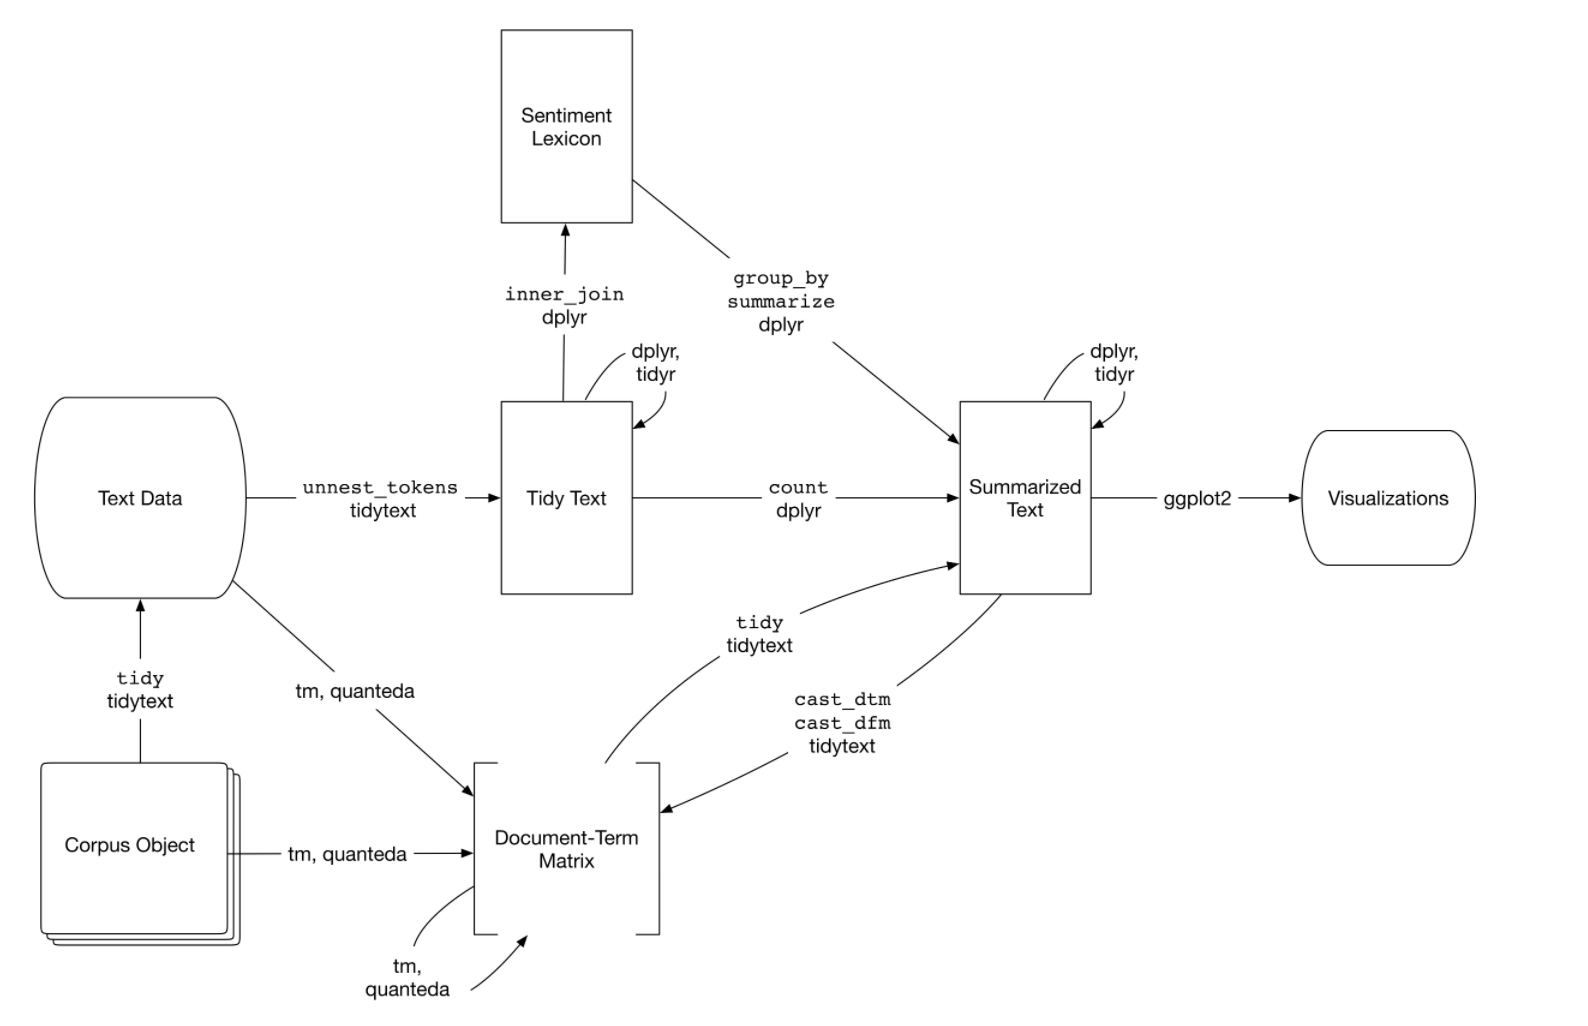
\includegraphics[width=22.06in]{flow chart}

\hypertarget{tidying-a-document-term-matrix}{%
\subsection{5.1 Tidying a document-term
matrix}\label{tidying-a-document-term-matrix}}

One of the most common structures that text mining packages work with is
the document-term matrix. The document-term matrix is a matrix where:

\begin{itemize}
\tightlist
\item
  Each row represents one documents
\item
  Each column represents one term
\item
  Each value (typically) contains the number of appearances of that term
  in that document.
\end{itemize}

Since most terms do not occur(they have the value zero), the
document-term matrix are usually implemented as sparse matrices.

document-term matrix object cannot be used directly with tidy tools, so
the tidytext package can convert between two formats.

\begin{itemize}
\tightlist
\item
  tidy() turns a document-term matrix into a tidy data frame.
\item
  cast() turns a tidy data frame into matrix. The tidytext provides
  three variation, each converting to a different type of matrix:

  \begin{itemize}
  \tightlist
  \item
    cast\_sparse() - convert to a sparse matrix
  \item
    cast\_dtm() - convert to a document-term matrix
  \item
    cast\_dfm() - convert to a dfm(document feature matrix) object
  \end{itemize}
\end{itemize}

A document-term matrix is typically comparable to a tidy data frame
after count or a group\_by/summarize that contains count or other
statistics for each combination of a term and document.

\hypertarget{tidying-documenttermmatrix-objects}{%
\subsection{5.1.5 Tidying DocumentTermMatrix
objects}\label{tidying-documenttermmatrix-objects}}

I was not able to find any data that is in the document-term matrix
form. So, I am using the data set provide in the text book.

\begin{Shaded}
\begin{Highlighting}[]
\KeywordTok{data}\NormalTok{(}\StringTok{"AssociatedPress"}\NormalTok{, }\DataTypeTok{package =} \StringTok{"topicmodels"}\NormalTok{)}
\NormalTok{AssociatedPress}
\end{Highlighting}
\end{Shaded}

\begin{verbatim}
## <<DocumentTermMatrix (documents: 2246, terms: 10473)>>
## Non-/sparse entries: 302031/23220327
## Sparsity           : 99%
## Maximal term length: 18
## Weighting          : term frequency (tf)
\end{verbatim}

There is 2246 documents and 10473 terms in the data set. We could see
the terms in the document with the Terms() function

\begin{Shaded}
\begin{Highlighting}[]
\NormalTok{terms <-}\StringTok{ }\KeywordTok{Terms}\NormalTok{(AssociatedPress)}
\KeywordTok{head}\NormalTok{(terms)}
\end{Highlighting}
\end{Shaded}

\begin{verbatim}
## [1] "aaron"      "abandon"    "abandoned"  "abandoning" "abbott"    
## [6] "abboud"
\end{verbatim}

We can turn the document-term matrix into a tidy data format by using
tidy()

\begin{Shaded}
\begin{Highlighting}[]
\NormalTok{tidy_data <-}\StringTok{ }\KeywordTok{tidy}\NormalTok{(AssociatedPress)}
\NormalTok{tidy_data}
\end{Highlighting}
\end{Shaded}

\begin{verbatim}
## # A tibble: 302,031 x 3
##    document term       count
##       <int> <chr>      <dbl>
##  1        1 adding         1
##  2        1 adult          2
##  3        1 ago            1
##  4        1 alcohol        1
##  5        1 allegedly      1
##  6        1 allen          1
##  7        1 apparently     2
##  8        1 appeared       1
##  9        1 arrested       1
## 10        1 assault        1
## # ... with 302,021 more rows
\end{verbatim}

We have three variables in the tidy\_data, document, term and count.
This is something that I am familiar with. We can perform sentiment
analysis or plot as we did in earlier chapter.

\begin{Shaded}
\begin{Highlighting}[]
\NormalTok{ap_sentiments_bing <-}\StringTok{ }\NormalTok{tidy_data }\OperatorTok
\StringTok{  }\KeywordTok{inner_join}\NormalTok{(}\KeywordTok{get_sentiments}\NormalTok{(}\StringTok{"bing"}\NormalTok{), }\DataTypeTok{by =} \KeywordTok{c}\NormalTok{(}\DataTypeTok{term =} \StringTok{"word"}\NormalTok{))}
\NormalTok{ap_sentiments_bing}
\end{Highlighting}
\end{Shaded}

\begin{verbatim}
## # A tibble: 30,094 x 4
##    document term    count sentiment
##       <int> <chr>   <dbl> <chr>    
##  1        1 assault     1 negative 
##  2        1 complex     1 negative 
##  3        1 death       1 negative 
##  4        1 died        1 negative 
##  5        1 good        2 positive 
##  6        1 illness     1 negative 
##  7        1 killed      2 negative 
##  8        1 like        2 positive 
##  9        1 liked       1 positive 
## 10        1 miracle     1 positive 
## # ... with 30,084 more rows
\end{verbatim}

\begin{Shaded}
\begin{Highlighting}[]
\NormalTok{ap_sentiments_afinn <-}\StringTok{ }\NormalTok{tidy_data }\OperatorTok
\StringTok{  }\KeywordTok{inner_join}\NormalTok{(}\KeywordTok{get_sentiments}\NormalTok{(}\StringTok{"afinn"}\NormalTok{), }\DataTypeTok{by =} \KeywordTok{c}\NormalTok{(}\DataTypeTok{term =} \StringTok{"word"}\NormalTok{))}
\NormalTok{ap_sentiments_afinn}
\end{Highlighting}
\end{Shaded}

\begin{verbatim}
## # A tibble: 31,665 x 4
##    document term     count value
##       <int> <chr>    <dbl> <dbl>
##  1        1 arrested     1    -3
##  2        1 big          1     1
##  3        1 charged      1    -3
##  4        1 charges      1    -2
##  5        1 crying       1    -2
##  6        1 death        1    -2
##  7        1 died         1    -3
##  8        1 felony       1    -3
##  9        1 fire         1    -2
## 10        1 fired        2    -2
## # ... with 31,655 more rows
\end{verbatim}

\begin{Shaded}
\begin{Highlighting}[]
\NormalTok{ap_sentiments_nrc <-}\StringTok{ }\NormalTok{tidy_data }\OperatorTok
\StringTok{  }\KeywordTok{inner_join}\NormalTok{(}\KeywordTok{get_sentiments}\NormalTok{(}\StringTok{"nrc"}\NormalTok{), }\DataTypeTok{by =} \KeywordTok{c}\NormalTok{(}\DataTypeTok{term =} \StringTok{"word"}\NormalTok{))}
\NormalTok{ap_sentiments_nrc}
\end{Highlighting}
\end{Shaded}

\begin{verbatim}
## # A tibble: 147,609 x 4
##    document term     count sentiment   
##       <int> <chr>    <dbl> <chr>       
##  1        1 assault      1 anger       
##  2        1 assault      1 fear        
##  3        1 assault      1 negative    
##  4        1 boy          4 disgust     
##  5        1 boy          4 negative    
##  6        1 building     1 positive    
##  7        1 church       1 anticipation
##  8        1 church       1 joy         
##  9        1 church       1 positive    
## 10        1 church       1 trust       
## # ... with 147,599 more rows
\end{verbatim}

First looking at the sentiments from bing package, we cab see the
postive or negative words in our data.

\begin{Shaded}
\begin{Highlighting}[]
\NormalTok{ap_sentiments_bing}\OperatorTok
\StringTok{  }\KeywordTok{count}\NormalTok{(sentiment, term, }\DataTypeTok{wt =}\NormalTok{ count) }\OperatorTok
\StringTok{  }\KeywordTok{filter}\NormalTok{(n }\OperatorTok{>=}\StringTok{ }\DecValTok{200}\NormalTok{) }\OperatorTok
\StringTok{  }\KeywordTok{mutate}\NormalTok{(}\DataTypeTok{n =} \KeywordTok{ifelse}\NormalTok{(sentiment }\OperatorTok{==}\StringTok{ "negative"}\NormalTok{, }\OperatorTok{-}\NormalTok{n, n)) }\OperatorTok
\StringTok{  }\KeywordTok{mutate}\NormalTok{(}\DataTypeTok{term =} \KeywordTok{reorder}\NormalTok{(term, n)) }\OperatorTok
\StringTok{  }\KeywordTok{ggplot}\NormalTok{(}\KeywordTok{aes}\NormalTok{(term, n, }\DataTypeTok{fill =}\NormalTok{ sentiment)) }\OperatorTok{+}
\StringTok{  }\KeywordTok{geom_bar}\NormalTok{(}\DataTypeTok{stat =} \StringTok{"identity"}\NormalTok{) }\OperatorTok{+}
\StringTok{  }\KeywordTok{ylab}\NormalTok{(}\StringTok{"Contribution to sentiment"}\NormalTok{) }\OperatorTok{+}
\StringTok{  }\KeywordTok{coord_flip}\NormalTok{()}
\end{Highlighting}
\end{Shaded}

\includegraphics{Reading-notes-chap-5-7_files/figure-latex/unnamed-chunk-6-1.pdf}

trying out theme\_minimal() and theme\_classic() and theme\_clean()

\begin{Shaded}
\begin{Highlighting}[]
\NormalTok{ap_sentiments_bing}\OperatorTok
\StringTok{  }\KeywordTok{count}\NormalTok{(sentiment, term, }\DataTypeTok{wt =}\NormalTok{ count) }\OperatorTok
\StringTok{  }\KeywordTok{ungroup}\NormalTok{() }\OperatorTok
\StringTok{  }\KeywordTok{filter}\NormalTok{(n }\OperatorTok{>=}\StringTok{ }\DecValTok{200}\NormalTok{) }\OperatorTok
\StringTok{  }\KeywordTok{mutate}\NormalTok{(}\DataTypeTok{n =} \KeywordTok{ifelse}\NormalTok{(sentiment }\OperatorTok{==}\StringTok{ "negative"}\NormalTok{, }\OperatorTok{-}\NormalTok{n, n)) }\OperatorTok
\StringTok{  }\KeywordTok{mutate}\NormalTok{(}\DataTypeTok{term =} \KeywordTok{reorder}\NormalTok{(term, n)) }\OperatorTok
\StringTok{  }\KeywordTok{ggplot}\NormalTok{(}\KeywordTok{aes}\NormalTok{(term, n, }\DataTypeTok{fill =}\NormalTok{ sentiment)) }\OperatorTok{+}
\StringTok{  }\KeywordTok{geom_bar}\NormalTok{(}\DataTypeTok{stat =} \StringTok{"identity"}\NormalTok{) }\OperatorTok{+}
\StringTok{  }\KeywordTok{ylab}\NormalTok{(}\StringTok{"Contribution to sentiment"}\NormalTok{) }\OperatorTok{+}
\StringTok{  }\KeywordTok{coord_flip}\NormalTok{()}\OperatorTok{+}
\StringTok{  }\KeywordTok{theme_minimal}\NormalTok{()}
\end{Highlighting}
\end{Shaded}

\includegraphics{Reading-notes-chap-5-7_files/figure-latex/unnamed-chunk-7-1.pdf}

\begin{Shaded}
\begin{Highlighting}[]
\NormalTok{ap_sentiments_bing}\OperatorTok
\StringTok{  }\KeywordTok{count}\NormalTok{(sentiment, term, }\DataTypeTok{wt =}\NormalTok{ count) }\OperatorTok
\StringTok{  }\KeywordTok{ungroup}\NormalTok{() }\OperatorTok
\StringTok{  }\KeywordTok{filter}\NormalTok{(n }\OperatorTok{>=}\StringTok{ }\DecValTok{200}\NormalTok{) }\OperatorTok
\StringTok{  }\KeywordTok{mutate}\NormalTok{(}\DataTypeTok{n =} \KeywordTok{ifelse}\NormalTok{(sentiment }\OperatorTok{==}\StringTok{ "negative"}\NormalTok{, }\OperatorTok{-}\NormalTok{n, n)) }\OperatorTok
\StringTok{  }\KeywordTok{mutate}\NormalTok{(}\DataTypeTok{term =} \KeywordTok{reorder}\NormalTok{(term, n)) }\OperatorTok
\StringTok{  }\KeywordTok{ggplot}\NormalTok{(}\KeywordTok{aes}\NormalTok{(term, n, }\DataTypeTok{fill =}\NormalTok{ sentiment)) }\OperatorTok{+}
\StringTok{  }\KeywordTok{geom_bar}\NormalTok{(}\DataTypeTok{stat =} \StringTok{"identity"}\NormalTok{) }\OperatorTok{+}
\StringTok{  }\KeywordTok{ylab}\NormalTok{(}\StringTok{"Contribution to sentiment"}\NormalTok{) }\OperatorTok{+}
\StringTok{  }\KeywordTok{coord_flip}\NormalTok{()}\OperatorTok{+}
\StringTok{  }\KeywordTok{theme_classic}\NormalTok{()}
\end{Highlighting}
\end{Shaded}

\includegraphics{Reading-notes-chap-5-7_files/figure-latex/unnamed-chunk-7-2.pdf}

\begin{Shaded}
\begin{Highlighting}[]
\NormalTok{ap_sentiments_bing}\OperatorTok
\StringTok{  }\KeywordTok{count}\NormalTok{(sentiment, term, }\DataTypeTok{wt =}\NormalTok{ count) }\OperatorTok
\StringTok{  }\KeywordTok{ungroup}\NormalTok{() }\OperatorTok
\StringTok{  }\KeywordTok{filter}\NormalTok{(n }\OperatorTok{>=}\StringTok{ }\DecValTok{200}\NormalTok{) }\OperatorTok
\StringTok{  }\KeywordTok{mutate}\NormalTok{(}\DataTypeTok{n =} \KeywordTok{ifelse}\NormalTok{(sentiment }\OperatorTok{==}\StringTok{ "negative"}\NormalTok{, }\OperatorTok{-}\NormalTok{n, n)) }\OperatorTok
\StringTok{  }\KeywordTok{mutate}\NormalTok{(}\DataTypeTok{term =} \KeywordTok{reorder}\NormalTok{(term, n)) }\OperatorTok
\StringTok{  }\KeywordTok{ggplot}\NormalTok{(}\KeywordTok{aes}\NormalTok{(term, n, }\DataTypeTok{fill =}\NormalTok{ sentiment)) }\OperatorTok{+}
\StringTok{  }\KeywordTok{geom_bar}\NormalTok{(}\DataTypeTok{stat =} \StringTok{"identity"}\NormalTok{) }\OperatorTok{+}
\StringTok{  }\KeywordTok{ylab}\NormalTok{(}\StringTok{"Contribution to sentiment"}\NormalTok{) }\OperatorTok{+}
\StringTok{  }\KeywordTok{coord_flip}\NormalTok{()}\OperatorTok{+}
\StringTok{  }\KeywordTok{theme_clean}\NormalTok{()}
\end{Highlighting}
\end{Shaded}

\includegraphics{Reading-notes-chap-5-7_files/figure-latex/unnamed-chunk-7-3.pdf}

\hypertarget{tidying-dfm-objects}{%
\subsection{5.1.2 Tidying dfm objects}\label{tidying-dfm-objects}}

Other text mining packages provide alternative implementations of
document-term matrices, such as the dfm (document-feature matrix) class.

There is no explanation for DFM, This is what I found on Google:
``refers to documents in rows and ``features'' as columns"

What is features in this context? What is the difference between DFM and
DTM?

I do not know how to turn data into DFM right now. So, I am using data
set from the text book

\begin{Shaded}
\begin{Highlighting}[]
\KeywordTok{data}\NormalTok{(}\StringTok{"data_corpus_inaugural"}\NormalTok{, }\DataTypeTok{package =} \StringTok{"quanteda"}\NormalTok{)}
\NormalTok{inaug_dfm <-}\StringTok{ }\NormalTok{quanteda}\OperatorTok{::}\KeywordTok{dfm}\NormalTok{(data_corpus_inaugural, }\DataTypeTok{verbose =} \OtherTok{FALSE}\NormalTok{)}
\NormalTok{inaug_dfm}
\end{Highlighting}
\end{Shaded}

\begin{verbatim}
## Document-feature matrix of: 58 documents, 9,360 features (91.8% sparse) and 4 docvars.
##                  features
## docs              fellow-citizens  of the senate and house representatives
##   1789-Washington               1  71 116      1  48     2               2
##   1793-Washington               0  11  13      0   2     0               0
##   1797-Adams                    3 140 163      1 130     0               2
##   1801-Jefferson                2 104 130      0  81     0               0
##   1805-Jefferson                0 101 143      0  93     0               0
##   1809-Madison                  1  69 104      0  43     0               0
##                  features
## docs              : among vicissitudes
##   1789-Washington 1     1            1
##   1793-Washington 1     0            0
##   1797-Adams      0     4            0
##   1801-Jefferson  1     1            0
##   1805-Jefferson  0     7            0
##   1809-Madison    0     0            0
## [ reached max_ndoc ... 52 more documents, reached max_nfeat ... 9,350 more features ]
\end{verbatim}

Use tidy() to turn the DFM into tidy format

\begin{Shaded}
\begin{Highlighting}[]
\NormalTok{inaug_td <-}\StringTok{ }\KeywordTok{tidy}\NormalTok{(inaug_dfm)}
\NormalTok{inaug_td}
\end{Highlighting}
\end{Shaded}

\begin{verbatim}
## # A tibble: 44,710 x 3
##    document        term            count
##    <chr>           <chr>           <dbl>
##  1 1789-Washington fellow-citizens     1
##  2 1797-Adams      fellow-citizens     3
##  3 1801-Jefferson  fellow-citizens     2
##  4 1809-Madison    fellow-citizens     1
##  5 1813-Madison    fellow-citizens     1
##  6 1817-Monroe     fellow-citizens     5
##  7 1821-Monroe     fellow-citizens     1
##  8 1841-Harrison   fellow-citizens    11
##  9 1845-Polk       fellow-citizens     1
## 10 1849-Taylor     fellow-citizens     1
## # ... with 44,700 more rows
\end{verbatim}

Now, we may perform tf\_idf calculation to see the important words in
each document.

\begin{Shaded}
\begin{Highlighting}[]
\NormalTok{inaug_tf_idf <-}\StringTok{ }\NormalTok{inaug_td }\OperatorTok
\StringTok{  }\KeywordTok{bind_tf_idf}\NormalTok{(term, document, count) }\OperatorTok
\StringTok{  }\KeywordTok{arrange}\NormalTok{(}\KeywordTok{desc}\NormalTok{(tf_idf))}

\NormalTok{inaug_tf_idf}
\end{Highlighting}
\end{Shaded}

\begin{verbatim}
## # A tibble: 44,710 x 6
##    document        term        count      tf   idf tf_idf
##    <chr>           <chr>       <dbl>   <dbl> <dbl>  <dbl>
##  1 1793-Washington arrive          1 0.00680  4.06 0.0276
##  2 1793-Washington upbraidings     1 0.00680  4.06 0.0276
##  3 1793-Washington violated        1 0.00680  3.37 0.0229
##  4 1793-Washington willingly       1 0.00680  3.37 0.0229
##  5 1793-Washington incurring       1 0.00680  3.37 0.0229
##  6 1793-Washington previous        1 0.00680  2.96 0.0201
##  7 1793-Washington knowingly       1 0.00680  2.96 0.0201
##  8 1793-Washington injunctions     1 0.00680  2.96 0.0201
##  9 1793-Washington witnesses       1 0.00680  2.96 0.0201
## 10 1793-Washington besides         1 0.00680  2.67 0.0182
## # ... with 44,700 more rows
\end{verbatim}

Visualize the words most specific to each document

\begin{Shaded}
\begin{Highlighting}[]
\NormalTok{inaug_tf_idf }\OperatorTok\StringTok{ }
\StringTok{  }\KeywordTok{group_by}\NormalTok{(document) }\OperatorTok\StringTok{ }
\StringTok{  }\KeywordTok{filter}\NormalTok{(document }\OperatorTok{==}\StringTok{ "1793-Washington"} \OperatorTok{|}\StringTok{ }\NormalTok{document }\OperatorTok{==}\StringTok{ "2009-Obama"}\NormalTok{) }\OperatorTok\StringTok{ }
\StringTok{  }\KeywordTok{top_n}\NormalTok{(}\DecValTok{20}\NormalTok{, tf_idf) }\OperatorTok\StringTok{ }
\StringTok{  }\KeywordTok{arrange}\NormalTok{(}\KeywordTok{desc}\NormalTok{(tf_idf)) }\OperatorTok\StringTok{ }
\StringTok{  }\KeywordTok{ungroup}\NormalTok{() }\OperatorTok\StringTok{ }
\StringTok{  }\KeywordTok{ggplot}\NormalTok{(}\KeywordTok{aes}\NormalTok{(term, tf_idf, }\DataTypeTok{fill =}\NormalTok{ document)) }\OperatorTok{+}
\StringTok{  }\KeywordTok{geom_col}\NormalTok{(}\DataTypeTok{show.legend =} \OtherTok{FALSE}\NormalTok{) }\OperatorTok{+}
\StringTok{  }\KeywordTok{labs}\NormalTok{(}\DataTypeTok{x =} \OtherTok{NULL}\NormalTok{, }\DataTypeTok{y =} \StringTok{"tf-idf"}\NormalTok{) }\OperatorTok{+}
\StringTok{  }\KeywordTok{facet_wrap}\NormalTok{(}\OperatorTok{~}\NormalTok{document, }\DataTypeTok{ncol =} \DecValTok{2}\NormalTok{, }\DataTypeTok{scales =} \StringTok{"free"}\NormalTok{) }\OperatorTok{+}
\StringTok{  }\KeywordTok{coord_flip}\NormalTok{()}
\end{Highlighting}
\end{Shaded}

\includegraphics{Reading-notes-chap-5-7_files/figure-latex/unnamed-chunk-11-1.pdf}
Notice that ``('' and ``)'' are mark as a term, in the data set. But
using unnest\_tokens will remove them.

We can also get a visualization of the changes in word usage from year
to year.

Firstly, get the year in the document variable

\begin{Shaded}
\begin{Highlighting}[]
\NormalTok{year_term_counts <-}\StringTok{ }\NormalTok{inaug_td }\OperatorTok
\StringTok{  }\KeywordTok{extract}\NormalTok{(document, }\StringTok{"year"}\NormalTok{, }\StringTok{"(}\CharTok{\textbackslash{}\textbackslash{}}\StringTok{d+)"}\NormalTok{, }\DataTypeTok{convert =} \OtherTok{TRUE}\NormalTok{) }\OperatorTok
\StringTok{  }\KeywordTok{complete}\NormalTok{(year, term, }\DataTypeTok{fill =} \KeywordTok{list}\NormalTok{(}\DataTypeTok{count =} \DecValTok{0}\NormalTok{)) }\OperatorTok
\StringTok{  }\KeywordTok{group_by}\NormalTok{(year) }\OperatorTok
\StringTok{  }\KeywordTok{mutate}\NormalTok{(}\DataTypeTok{year_total =} \KeywordTok{sum}\NormalTok{(count))}

\NormalTok{year_term_counts }\OperatorTok
\StringTok{  }\KeywordTok{filter}\NormalTok{(term }\OperatorTok\StringTok{ }\KeywordTok{c}\NormalTok{(}\StringTok{"america"}\NormalTok{, }\StringTok{"foreign"}\NormalTok{, }\StringTok{"freedom"}\NormalTok{)) }\OperatorTok
\StringTok{  }\KeywordTok{ggplot}\NormalTok{(}\KeywordTok{aes}\NormalTok{(year, count }\OperatorTok{/}\StringTok{ }\NormalTok{year_total)) }\OperatorTok{+}
\StringTok{  }\KeywordTok{geom_point}\NormalTok{() }\OperatorTok{+}
\StringTok{  }\KeywordTok{geom_smooth}\NormalTok{() }\OperatorTok{+}
\StringTok{  }\KeywordTok{facet_wrap}\NormalTok{(}\OperatorTok{~}\StringTok{ }\NormalTok{term, }\DataTypeTok{scales =} \StringTok{"free_y"}\NormalTok{) }\OperatorTok{+}
\StringTok{  }\KeywordTok{scale_y_continuous}\NormalTok{(}\DataTypeTok{labels =}\NormalTok{ scales}\OperatorTok{::}\KeywordTok{percent_format}\NormalTok{()) }\OperatorTok{+}
\StringTok{  }\KeywordTok{ylab}\NormalTok{(}\StringTok{"% frequency of word in inaugural address"}\NormalTok{)}
\end{Highlighting}
\end{Shaded}

\begin{verbatim}
## `geom_smooth()` using method = 'loess' and formula 'y ~ x'
\end{verbatim}

\includegraphics{Reading-notes-chap-5-7_files/figure-latex/unnamed-chunk-12-1.pdf}
\#\# 5.2 Casting tidy text data into a matrix Use cast\_dtm to cast a
tidy data into document-term matrix

\begin{Shaded}
\begin{Highlighting}[]
\NormalTok{tidy_data }\OperatorTok\StringTok{ }
\StringTok{  }\KeywordTok{cast_dtm}\NormalTok{(document, term, count)}
\end{Highlighting}
\end{Shaded}

\begin{verbatim}
## <<DocumentTermMatrix (documents: 2246, terms: 10473)>>
## Non-/sparse entries: 302031/23220327
## Sparsity           : 99%
## Maximal term length: 18
## Weighting          : term frequency (tf)
\end{verbatim}

We could also cast the tidy data into a document-feature matrix object
using cast\_dfm()

\begin{Shaded}
\begin{Highlighting}[]
\NormalTok{tidy_data }\OperatorTok\StringTok{ }
\StringTok{  }\KeywordTok{cast_dfm}\NormalTok{(document, term, count)}
\end{Highlighting}
\end{Shaded}

\begin{verbatim}
## Document-feature matrix of: 2,246 documents, 10,473 features (98.7% sparse).
##     features
## docs adding adult ago alcohol allegedly allen apparently appeared arrested
##    1      1     2   1       1         1     1          2        1        1
##    2      0     0   0       0         0     0          0        1        0
##    3      0     0   1       0         0     0          0        1        0
##    4      0     0   3       0         0     0          0        0        0
##    5      0     0   0       0         0     0          0        0        0
##    6      0     0   2       0         0     0          0        0        0
##     features
## docs assault
##    1       1
##    2       0
##    3       0
##    4       0
##    5       0
##    6       0
## [ reached max_ndoc ... 2,240 more documents, reached max_nfeat ... 10,463 more features ]
\end{verbatim}

We can also turn the news data in chap 1-4 into document-term matrix

\begin{Shaded}
\begin{Highlighting}[]
\NormalTok{newsdata <-}\StringTok{ }\KeywordTok{c}\NormalTok{(}\StringTok{"Some provinces are scrambling to increase testing capacity as coronavirus infections spike across Canada and lineups at COVID-19 testing sites see a significant influx of people. }

\StringTok{In order to accommodate demand, opening hours at two Ottawa assessment centres will be extended in the coming days, Ottawa Public Health, Children's Hospital of Eastern Ontario and Ottawa Hospital said in a joint statement Monday afternoon. }

\StringTok{The statement said the health authorities are hiring more staff and training them so that the Brewer assessment centre can accept patients for 12 hours per day, seven days a week — four more hours per day than it is normally open.}

\StringTok{We knew that with the kids returning to school we would see these volumes. To prepare, we have tripled staffing in the last month for testing children and youth at the [Brewer Arena assessment centre]. More are being trained and still more are being hired, the statement said. As of 3:15 p.m. ET on Tuesday, Canada had 138,572 confirmed or presumptive coronavirus cases. Provinces and territories listed 121,555 of those as recovered or resolved. A CBC News tally of deaths based on provincial reports, regional health information and CBC's reporting stood at 9,226.}

\StringTok{At a news conference Tuesday, Ontario Premier Doug Ford said the coronavirus is continuing to spread.}

\StringTok{The province announced 251 new cases Tuesday, with the majority of those cases found in Toronto, Ottawa and Peel region with 73, 51 and 42 cases, respectively. }

\StringTok{As we see around the world, countries are getting hammered by COVID-19, said Ford.}

\StringTok{He also said he believes a second wave of the virus is coming to the province and said officials are cautioning that the second wave could be more complicated than the first one. Ford said Ontario is now expanding testing and building up a supply of personal protective equipment in anticipation of a continued spike in cases. }

\StringTok{At an Ottawa council meeting last Wednesday, elected officials from across the city called for an expansion of its testing system to better meet demand.}

\StringTok{Part of our future success will depend on our ability to test, to test rapidly and to remove barriers to access to testing, said Rideau-Vanier Coun. Mathieu Fleury in an interview with CBC.}

\StringTok{In London, Ont., a long line of cars was seen waiting outside the city's only open assessment centre — the Carling Heights Optimist Centre — on Sunday.}

\StringTok{The Middlesex-London Health Unit said the lengthy wait was partly due to a staffing shortage at that location.}

\StringTok{Many of the cars in line at the Carling Heights Optimist Centre were filled with young people looking to get tested.Quebec recorded 291 new cases of COVID-19 on Tuesday, which is the sixth day in a row the province has reported more than 200 cases.}

\StringTok{In response to the rising number of infections, Quebec Premier François Legault warned the public that social gatherings must be limited immediately in order to avoid closing schools and businesses.}

\StringTok{The situation is critical. It's worrisome, and we must act now, he said at a news conference Tuesday. Legault also said Quebec faces a real risk of a second wave.}

\StringTok{Quebec City and the Lower Saint-Lawrence regions are being closely monitored and may be moved to the orange alert level, up from yellow, indicating an increased risk of COVID-19 to the public, sources told Radio-Canada.}

\StringTok{Health Minister Christian Dubé said at the same news conference that an orange classification would mean the closure of bars and reducing the number of people allowed in private gatherings from 10 to six. At the federal level, Chief Public Health Officer Dr. Theresa Tam said Tuesday that the government is currently working closely with provincial microbiology labs to enhance test processing capacity. }

\StringTok{Tam told reporters that the current national capacity is beyond 60,000 [tests per day] at the national level.  }

\StringTok{She said Canada needs to augment the portfolio of testing capabilities in Canada to include new technology like rapid saliva tests.  }

\StringTok{Testing issues have also been reported in St. John's, with local mother Flora Salvo saying she spent four days on the phone trying to book a COVID-19 test and that the reservation system needs to be revamped.}

\StringTok{She said the painfully slow process of getting tested — from her first call to when she received a negative result last Saturday — stretched over a full week. }
\StringTok{"}\NormalTok{ ,}

\StringTok{"TORONTO -- Rising numbers of COVID-19 cases in multiple provinces are stoking fears of a potential second wave, and one infectious disease expert says this surge in infections might 'very well' be the start of that next phase in the pandemic.}

\StringTok{Infectious disease specialist Dr. Isaac Bogoch says that current upward trends in B.C., Alberta, Manitoba, Ontario and Quebec may be fuelling Canada’s second wave of coronavirus infections.}

\StringTok{It might be, it very well might be. We're certainly seeing these cases rumble up in the wrong direction, and quite frankly what happens over the next few weeks and then over the next month or two ahead really depends on us. If we let our guard down as citizens, if we let our guard down for example as businesses and organizations, then we'll see a spike in cases, Bogoch told CTV's Your Morning on Tuesday.}
\StringTok{"}\NormalTok{, }

\StringTok{"}
\StringTok{Knoxdale-Merivale councillor and Ottawa Board of Health chair Keith Egli said Tuesday that school reopenings remain a priority, particularly in light of concerns over children’s mental health and emotional well-being during the past six months.}

\StringTok{“All society is impacted when people cannot rely on schools to support childhood development and economic activity,” he said, adding that Ottawa Public Health has prioritized working with school boards to help ensure a successful return to classes, meeting weekly to review plans and feedback, and provide guidance.}

\StringTok{Dr. Etches also addressed the possibility, raised earlier in the day by Ontario Premier Doug Ford, of the province’s returning to stricter measures and lockdowns to help contain the spread of COVID-19, especially in current hotspots such as Ottawa, Toronto and the Peel region.}

\StringTok{“We’re in favour of a risk-based approach, absolutely. We know that larger centres are always going to have a greater risk of transmission of COVID, for many reasons — density of population and sheer numbers of people — so we absolutely support an approach based on risk.”}

\StringTok{Ottawa will be expanding the hours and capacity of its care clinics and COVID-19 assessment centres, as school reopenings have led to greatly increased lineups and wait times at those sites, particular at Brewer Arena.}

\StringTok{Dr. Alan Forster, the testing strategy lead with the Champlain COVID-19 Response Committee, made the announcement Tuesday, indicating that the levels of testing in the area, currently at about 2,000 per day, could increase to 3,000 with increased hours and staffing, and as much as 3,500 if mobile testing in schools and other such venues is added.}


\StringTok{Forster said he expects that Brewer Arena and the Coventry Road sites will increase from eight hours a day to 12, seven days a week. Care clinics operated by the Queensway-Carleton and Montfort hospitals will expand their weekend hours.}

\StringTok{The changes, he added, are expected to take place in the next week.}

\StringTok{Yet Ottawa’s chief medical officer of health, Dr. Vera Etches, urged residents to only seek out testing if they display symptoms of have come in direct contact with those who have tested positive.}

\StringTok{Instead, she recommended that people reexamine and possibly modify their behaviours to ensure they’re limiting the number of close contacts in their circle and following other precautions, including avoiding large social gatherings.}

\StringTok{“There is potential harm when the value of asymptomatic testing is low, and it’s displacing people who need to have a test,” said Etches. “And the labs need to be able to turn around the results quickly for controlled outbreaks and school-setting investigations.”}

\StringTok{Etches reinforced Ottawa Public Heath’s position that social networks, and not businesses, are largely driving infections up. Most of the cases, she said, are related to outbreaks, such as those at long-term care facilities, or, in about one-quarter of cases, of unknown origin.}

\StringTok{“The rest of the cases are what we call sporadic, either usually linked to a household close contact or a social group close contact. That is the most common source of exposure.}

\StringTok{“We have very few workplace outbreaks that have been identified,” she added, “but we know everything’s connected.}

\StringTok{“The call today is for each of us to think about how many close contacts did you have this week where you were within two metres, especially indoors without a mask on? In each of those situations, that could be connected to a chain of transmission.}

\StringTok{“We want everybody to do their part to decrease those numbers of close contacts in our lives.”}

\StringTok{Ottawa reported 52 new cases of COVID-19 on Tuesday, down from 61 reported Monday.}

\StringTok{Five residents at West End Villa long-term care home have died from complications resulting from COVID-19.}

\StringTok{Extendicare, which manages the facility, confirmed the deaths in a statement from West End Villa administrator Kelly Keller on Monday.}

\StringTok{One of the deaths had previously been reported.}

\StringTok{“We are deeply saddened to share that as of September 14, five of our residents have passed away from complications related to COVID-19,” Keller wrote in statement. “We have been in contact with the families of these residents and offer them our condolences in this difficult time. All families with loved ones at Extendicare West End Villa have also been informed.}

\StringTok{“We cannot comment further on our residents out of respect for their privacy and the privacy of their families.”}

\StringTok{The 242-bed Elmira Avenue facility was listed as being in outbreak status by Ottawa Public Health effective Aug. 30. According to the province’s latest figures, 46 residents and nine staff members have tested positive.}

\StringTok{Advertisement}
\StringTok{Article content continued}
\StringTok{“We have conducted a second round of COVID-19 surveillance testing to help ensure our cohorting efforts are as effective as possible,” added Keller, “and we expect to receive the results of those tests over the coming days.}

\StringTok{Ottawa Public Health reported 52 new COVID-19 cases and four new deaths Tuesday, bringing those totals to 3,335 and 272, respectively.}

\StringTok{Nine Ottawa residents are currently hospitalized with COVID-19, but none are in intensive care.}

\StringTok{There are currently 362 active cases in Ottawa, while 2,753 have been resolved.}

\StringTok{Additionally, OPH confirms 19 health-care or child-care establishments with outbreaks, an increase of one from Monday’s report. The most recent addition to OPH’s institutional outbreak list is Riverview Development Services, which reported one staff case.}

\StringTok{Meanwhile, two more Ottawa French-language schools have reported people who have COVID-19, bringing the total number of people testing positive to 11 at nine Ottawa schools.}

\StringTok{The new Ottawa schools identified in the provincial database on Tuesday are Marius-Barbeau elementary, with one case, and Gabrielle-Roy elementary, with two cases. All three individuals were not staff or students, but are listed as “other.”}

\StringTok{Provincial}

\StringTok{Ontario Premier Doug Ford hinted on Tuesday that the province may soon offer asymptomatic COVID-19 testing through pharmacies such as Shopper’s Drug Mart.}

\StringTok{Citing the long lineups for testing, particularly after school openings in the province have prompted more people to seek testing, Ford indicated that he spoke earlier in the day with the CEO of Shopper’s, and that an announcement on the matter is forthcoming.}

\StringTok{“You’ll be hearing from us over the next couple of days,” Ford said. “I just want to make sure that all the ducks are in a row and then we’ll make an announcement.}

\StringTok{“I’m not going to say that 100 per cent, but we’re all over it.”}

\StringTok{The premier also would not rule out the possibility of the province further clamping down on social gatherings to help stem the recent increase in COVID-19 cases, indicating that he’s been in talks with Ottawa Mayor Jim Watson, Toronto Mayor John Tory and Brampton Mayor Patrick Brown to get their input on the issue."}\NormalTok{)}

\NormalTok{newsdata}
\end{Highlighting}
\end{Shaded}

\begin{verbatim}
## [1] "Some provinces are scrambling to increase testing capacity as coronavirus infections spike across Canada and lineups at COVID-19 testing sites see a significant influx of people. \n\nIn order to accommodate demand, opening hours at two Ottawa assessment centres will be extended in the coming days, Ottawa Public Health, Children's Hospital of Eastern Ontario and Ottawa Hospital said in a joint statement Monday afternoon. \n\nThe statement said the health authorities are hiring more staff and training them so that the Brewer assessment centre can accept patients for 12 hours per day, seven days a week — four more hours per day than it is normally open.\n\nWe knew that with the kids returning to school we would see these volumes. To prepare, we have tripled staffing in the last month for testing children and youth at the [Brewer Arena assessment centre]. More are being trained and still more are being hired, the statement said. As of 3:15 p.m. ET on Tuesday, Canada had 138,572 confirmed or presumptive coronavirus cases. Provinces and territories listed 121,555 of those as recovered or resolved. A CBC News tally of deaths based on provincial reports, regional health information and CBC's reporting stood at 9,226.\n\nAt a news conference Tuesday, Ontario Premier Doug Ford said the coronavirus is continuing to spread.\n\nThe province announced 251 new cases Tuesday, with the majority of those cases found in Toronto, Ottawa and Peel region with 73, 51 and 42 cases, respectively. \n\nAs we see around the world, countries are getting hammered by COVID-19, said Ford.\n\nHe also said he believes a second wave of the virus is coming to the province and said officials are cautioning that the second wave could be more complicated than the first one. Ford said Ontario is now expanding testing and building up a supply of personal protective equipment in anticipation of a continued spike in cases. \n\nAt an Ottawa council meeting last Wednesday, elected officials from across the city called for an expansion of its testing system to better meet demand.\n\nPart of our future success will depend on our ability to test, to test rapidly and to remove barriers to access to testing, said Rideau-Vanier Coun. Mathieu Fleury in an interview with CBC.\n\nIn London, Ont., a long line of cars was seen waiting outside the city's only open assessment centre — the Carling Heights Optimist Centre — on Sunday.\n\nThe Middlesex-London Health Unit said the lengthy wait was partly due to a staffing shortage at that location.\n\nMany of the cars in line at the Carling Heights Optimist Centre were filled with young people looking to get tested.Quebec recorded 291 new cases of COVID-19 on Tuesday, which is the sixth day in a row the province has reported more than 200 cases.\n\nIn response to the rising number of infections, Quebec Premier François Legault warned the public that social gatherings must be limited immediately in order to avoid closing schools and businesses.\n\nThe situation is critical. It's worrisome, and we must act now, he said at a news conference Tuesday. Legault also said Quebec faces a real risk of a second wave.\n\nQuebec City and the Lower Saint-Lawrence regions are being closely monitored and may be moved to the orange alert level, up from yellow, indicating an increased risk of COVID-19 to the public, sources told Radio-Canada.\n\nHealth Minister Christian Dubé said at the same news conference that an orange classification would mean the closure of bars and reducing the number of people allowed in private gatherings from 10 to six. At the federal level, Chief Public Health Officer Dr. Theresa Tam said Tuesday that the government is currently working closely with provincial microbiology labs to enhance test processing capacity. \n\nTam told reporters that the current national capacity is beyond 60,000 [tests per day] at the national level.  \n\nShe said Canada needs to augment the portfolio of testing capabilities in Canada to include new technology like rapid saliva tests.  \n\nTesting issues have also been reported in St. John's, with local mother Flora Salvo saying she spent four days on the phone trying to book a COVID-19 test and that the reservation system needs to be revamped.\n\nShe said the painfully slow process of getting tested — from her first call to when she received a negative result last Saturday — stretched over a full week. \n"                                                                                                                                                                                                                                                                                                                                                                                                                                                                                                                                                                                                                                                                                                                                                                                                                                                                                                                                                                                                                                                                                                                                                                                                                                                                                                                                                                                                                                                                                                                                                                                                                                                                                                                                                                                                                                                                                                                                                                                                                                                                                                                                                                                                                                                                                                                                                                                                                                                                                                                                                                                                                                                                                       
## [2] "TORONTO -- Rising numbers of COVID-19 cases in multiple provinces are stoking fears of a potential second wave, and one infectious disease expert says this surge in infections might 'very well' be the start of that next phase in the pandemic.\n\nInfectious disease specialist Dr. Isaac Bogoch says that current upward trends in B.C., Alberta, Manitoba, Ontario and Quebec may be fuelling Canada’s second wave of coronavirus infections.\n\nIt might be, it very well might be. We're certainly seeing these cases rumble up in the wrong direction, and quite frankly what happens over the next few weeks and then over the next month or two ahead really depends on us. If we let our guard down as citizens, if we let our guard down for example as businesses and organizations, then we'll see a spike in cases, Bogoch told CTV's Your Morning on Tuesday.\n"                                                                                                                                                                                                                                                                                                                                                                                                                                                                                                                                                                                                                                                                                                                                                                                                                                                                                                                                                                                                                                                                                                                                                                                                                                                                                                                                                                                                                                                                                                                                                                                                                                                                                                                                                                                                                                                                                                                                                                                                                                                                                                                                                                                                                                                                                                                                                                                                                                                                                                                                                                                                                                                                                                                                                                                                                                                                                                                                                                                                                                                                                                                                                                                                                                                                                                                                                                                                                                                                                                                                                                                                                                                                                                                                                                                                                                                                                                                                                                                                                                                                                                                                                                                                                                                                                                                                                                                                                                                                                                                                                                                                                                                                                                                                                                                                                                                                                                                                                                                                                                                                                                                                                                                                                                                                                                                                                                                                                                                                                                                                                                                                                                                                                                                                                                                                                                                                                                                                                                                                                                                                                                                                                                                                                                                                                                                                                                                                   
## [3] "\nKnoxdale-Merivale councillor and Ottawa Board of Health chair Keith Egli said Tuesday that school reopenings remain a priority, particularly in light of concerns over children’s mental health and emotional well-being during the past six months.\n\n“All society is impacted when people cannot rely on schools to support childhood development and economic activity,” he said, adding that Ottawa Public Health has prioritized working with school boards to help ensure a successful return to classes, meeting weekly to review plans and feedback, and provide guidance.\n\nDr. Etches also addressed the possibility, raised earlier in the day by Ontario Premier Doug Ford, of the province’s returning to stricter measures and lockdowns to help contain the spread of COVID-19, especially in current hotspots such as Ottawa, Toronto and the Peel region.\n\n“We’re in favour of a risk-based approach, absolutely. We know that larger centres are always going to have a greater risk of transmission of COVID, for many reasons — density of population and sheer numbers of people — so we absolutely support an approach based on risk.”\n\nOttawa will be expanding the hours and capacity of its care clinics and COVID-19 assessment centres, as school reopenings have led to greatly increased lineups and wait times at those sites, particular at Brewer Arena.\n\nDr. Alan Forster, the testing strategy lead with the Champlain COVID-19 Response Committee, made the announcement Tuesday, indicating that the levels of testing in the area, currently at about 2,000 per day, could increase to 3,000 with increased hours and staffing, and as much as 3,500 if mobile testing in schools and other such venues is added.\n\n\nForster said he expects that Brewer Arena and the Coventry Road sites will increase from eight hours a day to 12, seven days a week. Care clinics operated by the Queensway-Carleton and Montfort hospitals will expand their weekend hours.\n\nThe changes, he added, are expected to take place in the next week.\n\nYet Ottawa’s chief medical officer of health, Dr. Vera Etches, urged residents to only seek out testing if they display symptoms of have come in direct contact with those who have tested positive.\n\nInstead, she recommended that people reexamine and possibly modify their behaviours to ensure they’re limiting the number of close contacts in their circle and following other precautions, including avoiding large social gatherings.\n\n“There is potential harm when the value of asymptomatic testing is low, and it’s displacing people who need to have a test,” said Etches. “And the labs need to be able to turn around the results quickly for controlled outbreaks and school-setting investigations.”\n\nEtches reinforced Ottawa Public Heath’s position that social networks, and not businesses, are largely driving infections up. Most of the cases, she said, are related to outbreaks, such as those at long-term care facilities, or, in about one-quarter of cases, of unknown origin.\n\n“The rest of the cases are what we call sporadic, either usually linked to a household close contact or a social group close contact. That is the most common source of exposure.\n\n“We have very few workplace outbreaks that have been identified,” she added, “but we know everything’s connected.\n\n“The call today is for each of us to think about how many close contacts did you have this week where you were within two metres, especially indoors without a mask on? In each of those situations, that could be connected to a chain of transmission.\n\n“We want everybody to do their part to decrease those numbers of close contacts in our lives.”\n\nOttawa reported 52 new cases of COVID-19 on Tuesday, down from 61 reported Monday.\n\nFive residents at West End Villa long-term care home have died from complications resulting from COVID-19.\n\nExtendicare, which manages the facility, confirmed the deaths in a statement from West End Villa administrator Kelly Keller on Monday.\n\nOne of the deaths had previously been reported.\n\n“We are deeply saddened to share that as of September 14, five of our residents have passed away from complications related to COVID-19,” Keller wrote in statement. “We have been in contact with the families of these residents and offer them our condolences in this difficult time. All families with loved ones at Extendicare West End Villa have also been informed.\n\n“We cannot comment further on our residents out of respect for their privacy and the privacy of their families.”\n\nThe 242-bed Elmira Avenue facility was listed as being in outbreak status by Ottawa Public Health effective Aug. 30. According to the province’s latest figures, 46 residents and nine staff members have tested positive.\n\nAdvertisement\nArticle content continued\n“We have conducted a second round of COVID-19 surveillance testing to help ensure our cohorting efforts are as effective as possible,” added Keller, “and we expect to receive the results of those tests over the coming days.\n\nOttawa Public Health reported 52 new COVID-19 cases and four new deaths Tuesday, bringing those totals to 3,335 and 272, respectively.\n\nNine Ottawa residents are currently hospitalized with COVID-19, but none are in intensive care.\n\nThere are currently 362 active cases in Ottawa, while 2,753 have been resolved.\n\nAdditionally, OPH confirms 19 health-care or child-care establishments with outbreaks, an increase of one from Monday’s report. The most recent addition to OPH’s institutional outbreak list is Riverview Development Services, which reported one staff case.\n\nMeanwhile, two more Ottawa French-language schools have reported people who have COVID-19, bringing the total number of people testing positive to 11 at nine Ottawa schools.\n\nThe new Ottawa schools identified in the provincial database on Tuesday are Marius-Barbeau elementary, with one case, and Gabrielle-Roy elementary, with two cases. All three individuals were not staff or students, but are listed as “other.”\n\nProvincial\n\nOntario Premier Doug Ford hinted on Tuesday that the province may soon offer asymptomatic COVID-19 testing through pharmacies such as Shopper’s Drug Mart.\n\nCiting the long lineups for testing, particularly after school openings in the province have prompted more people to seek testing, Ford indicated that he spoke earlier in the day with the CEO of Shopper’s, and that an announcement on the matter is forthcoming.\n\n“You’ll be hearing from us over the next couple of days,” Ford said. “I just want to make sure that all the ducks are in a row and then we’ll make an announcement.\n\n“I’m not going to say that 100 per cent, but we’re all over it.”\n\nThe premier also would not rule out the possibility of the province further clamping down on social gatherings to help stem the recent increase in COVID-19 cases, indicating that he’s been in talks with Ottawa Mayor Jim Watson, Toronto Mayor John Tory and Brampton Mayor Patrick Brown to get their input on the issue."
\end{verbatim}

\begin{Shaded}
\begin{Highlighting}[]
\NormalTok{news_word <-}\StringTok{ }\KeywordTok{tibble}\NormalTok{(}\DataTypeTok{article =} \KeywordTok{c}\NormalTok{(}\StringTok{"1"}\NormalTok{, }\StringTok{"2"}\NormalTok{,}\StringTok{"3"}\NormalTok{), }\DataTypeTok{text =}\NormalTok{ newsdata)}
\NormalTok{news_word}
\end{Highlighting}
\end{Shaded}

\begin{verbatim}
## # A tibble: 3 x 2
##   article text                                                             
##   <chr>   <chr>                                                            
## 1 1       "Some provinces are scrambling to increase testing capacity as c~
## 2 2       "TORONTO -- Rising numbers of COVID-19 cases in multiple provinc~
## 3 3       "\nKnoxdale-Merivale councillor and Ottawa Board of Health chair~
\end{verbatim}

\begin{Shaded}
\begin{Highlighting}[]
\NormalTok{news_dtm <-}\StringTok{ }\NormalTok{news_word }\OperatorTok
\StringTok{  }\KeywordTok{unnest_tokens}\NormalTok{(word, text) }\OperatorTok
\StringTok{  }\KeywordTok{anti_join}\NormalTok{(stop_words) }\OperatorTok\StringTok{ }
\StringTok{  }\KeywordTok{count}\NormalTok{(article, word) }\OperatorTok
\StringTok{  }\KeywordTok{cast_dtm}\NormalTok{(article, word, n)}
\end{Highlighting}
\end{Shaded}

\begin{verbatim}
## Joining, by = "word"
\end{verbatim}

\begin{Shaded}
\begin{Highlighting}[]
\NormalTok{news_dtm}
\end{Highlighting}
\end{Shaded}

\begin{verbatim}
## <<DocumentTermMatrix (documents: 3, terms: 567)>>
## Non-/sparse entries: 652/1049
## Sparsity           : 62%
## Maximal term length: 14
## Weighting          : term frequency (tf)
\end{verbatim}

\hypertarget{tidying-corpus-objects-with-metadata}{%
\subsection{5.3 Tidying corpus objects with
metadata}\label{tidying-corpus-objects-with-metadata}}

Some data structures are designed to store document collections before
tokenization, often called a ``corpus''. A corpus object is structured
like a list, with each item containing both text and metadata(infomation
such as the author, id, language).

We can also turn corpus into tidy format by using tidy(), and perform
any text mining techniques such as sentiment analysis and tf-idf.

\hypertarget{example-mining-financial-articles}{%
\subsection{5.3.1 Example: mining financial
articles}\label{example-mining-financial-articles}}

The data in tm.plugin.webmining allows us to retrieve the 20 most recent
articles related to Microsoft or other company's stock. Thus, the data
set that I am retrieved is different from the data set used in the
textbook. I an only looking at the article from Microsoft, Apple and
Google

\begin{Shaded}
\begin{Highlighting}[]
\KeywordTok{library}\NormalTok{(tm.plugin.webmining)}
\end{Highlighting}
\end{Shaded}

\begin{verbatim}
## Warning: package 'tm.plugin.webmining' was built under R version 3.6.3
\end{verbatim}

\begin{verbatim}
## 
## Attaching package: 'tm.plugin.webmining'
\end{verbatim}

\begin{verbatim}
## The following object is masked from 'package:tidyr':
## 
##     extract
\end{verbatim}

\begin{verbatim}
## The following object is masked from 'package:base':
## 
##     parse
\end{verbatim}

\begin{Shaded}
\begin{Highlighting}[]
\KeywordTok{library}\NormalTok{(purrr)}
\end{Highlighting}
\end{Shaded}

\begin{verbatim}
## Warning: package 'purrr' was built under R version 3.6.3
\end{verbatim}

\begin{verbatim}
## 
## Attaching package: 'purrr'
\end{verbatim}

\begin{verbatim}
## The following object is masked from 'package:rtweet':
## 
##     flatten
\end{verbatim}

\begin{Shaded}
\begin{Highlighting}[]
\NormalTok{company <-}\StringTok{ }\KeywordTok{c}\NormalTok{(}\StringTok{"Microsoft"}\NormalTok{, }\StringTok{"Apple"}\NormalTok{, }\StringTok{"Google"}\NormalTok{)}
\NormalTok{symbol <-}\StringTok{ }\KeywordTok{c}\NormalTok{(}\StringTok{"MSFT"}\NormalTok{, }\StringTok{"AAPL"}\NormalTok{, }\StringTok{"GOOG"}\NormalTok{)}

\NormalTok{download_articles <-}\StringTok{ }\ControlFlowTok{function}\NormalTok{(symbol) \{}
    \KeywordTok{WebCorpus}\NormalTok{(}\KeywordTok{YahooNewsSource}\NormalTok{(symbol))}
\NormalTok{\}}


\NormalTok{stock_articles <-}\StringTok{ }\KeywordTok{tibble}\NormalTok{(}\DataTypeTok{company =}\NormalTok{ company,}\DataTypeTok{symbol =}\NormalTok{ symbol) }\OperatorTok\StringTok{  }
\StringTok{  }\KeywordTok{mutate}\NormalTok{(}\DataTypeTok{corpus =} \KeywordTok{map}\NormalTok{(symbol, download_articles))}
\NormalTok{stock_articles}
\end{Highlighting}
\end{Shaded}

\begin{verbatim}
## # A tibble: 3 x 3
##   company   symbol corpus    
##   <chr>     <chr>  <list>    
## 1 Microsoft MSFT   <WebCorps>
## 2 Apple     AAPL   <WebCorps>
## 3 Google    GOOG   <WebCorps>
\end{verbatim}

Each of the item in corpus column is a WebCorpus object, which is a
special case of a corpus. We use tidy() to turn it into tidy format,
unnest it with unnest(), then tokenize with unnest\_tokens()

\begin{Shaded}
\begin{Highlighting}[]
\NormalTok{stock_tokens <-}\StringTok{ }\NormalTok{stock_articles }\OperatorTok
\StringTok{  }\KeywordTok{mutate}\NormalTok{(}\DataTypeTok{corpus =} \KeywordTok{map}\NormalTok{(corpus, tidy)) }\OperatorTok
\StringTok{  }\KeywordTok{unnest}\NormalTok{(}\DataTypeTok{cols =}\NormalTok{ (corpus))}

\NormalTok{stock_tokens}
\end{Highlighting}
\end{Shaded}

\begin{verbatim}
## # A tibble: 0 x 2
## # ... with 2 variables: company <chr>, symbol <chr>
\end{verbatim}

\hypertarget{summary}{%
\subsection{Summary}\label{summary}}

Text data may be organized in many different format for different
purpose, we may need to convert it between different form. For example,
converting tidy text data fram into document-term matrices.

Reflection!

\hypertarget{topic-modeling}{%
\subsection{6 Topic modeling}\label{topic-modeling}}

When we have collections of documents, we may want to divide into
natural groups so that we can understand them separately. Topic modeling
is a method for unsupervised classification of such documents, similar
to clustering.

Laten Dirichlet allocation (LDA) is a popular method for fitting a topic
model. LDA treats each document as a mixture of topics, and each topic
contains mixture of words. This allows documents to have same terms,
rather than separate each term into discrete groups.

A updated flow chart:

\begin{Shaded}
\begin{Highlighting}[]
\NormalTok{knitr}\OperatorTok{::}\KeywordTok{include_graphics}\NormalTok{(}\StringTok{'flow chart 2.png'}\NormalTok{)}
\end{Highlighting}
\end{Shaded}

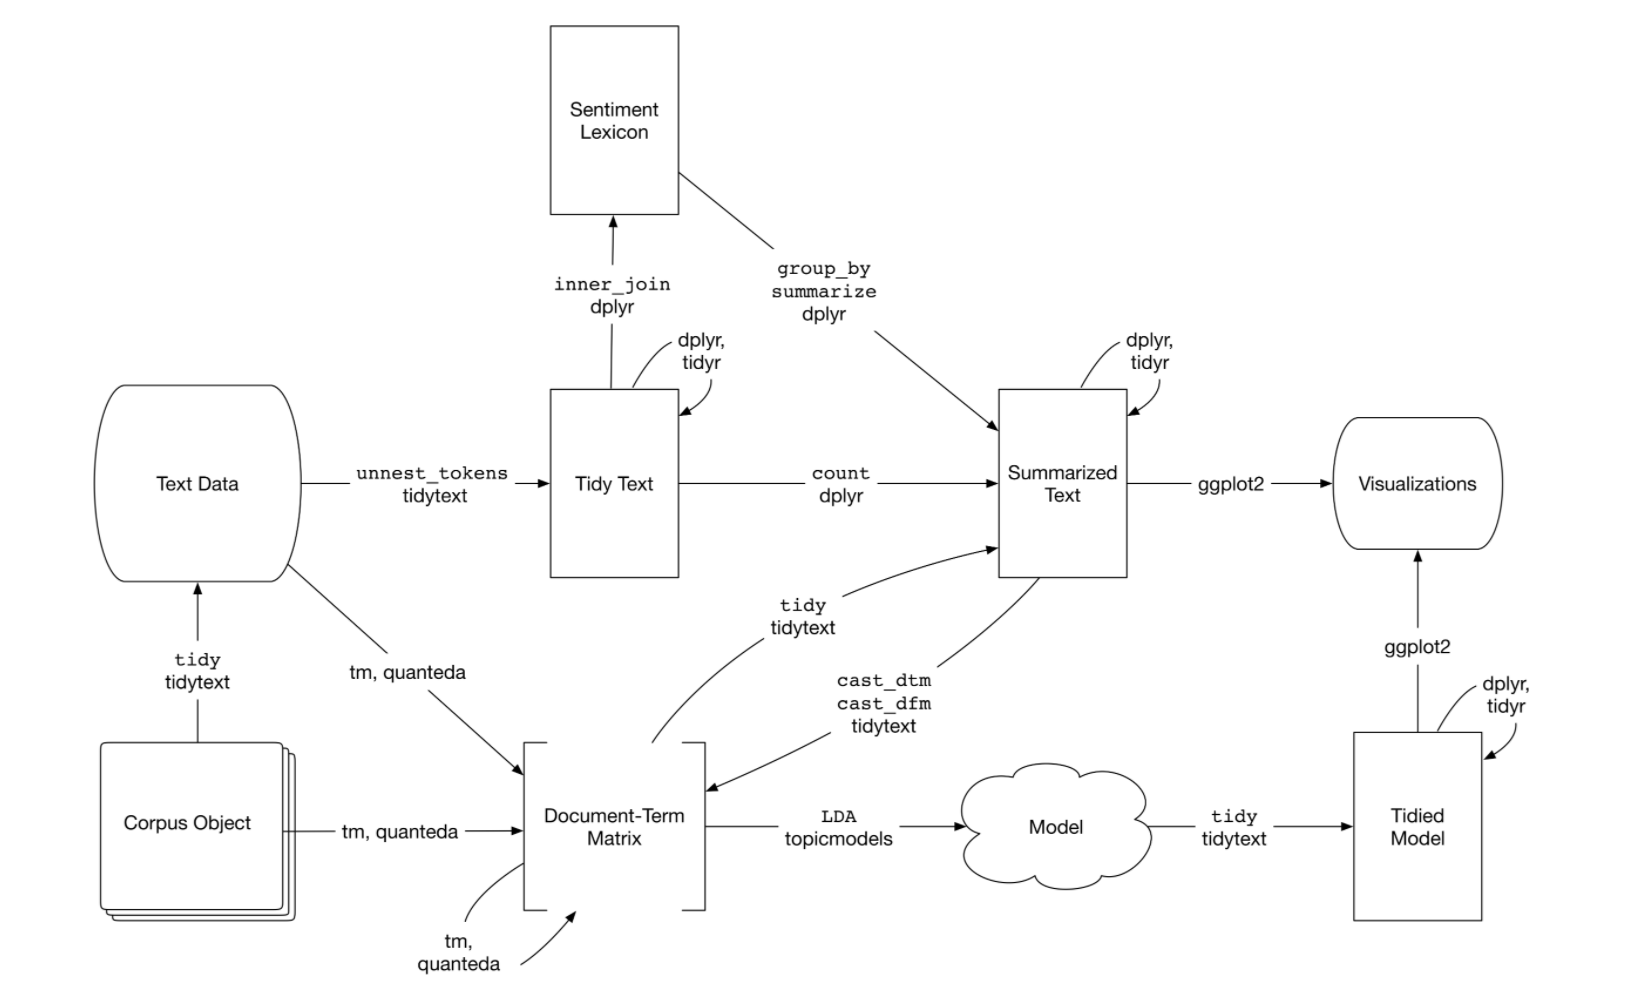
\includegraphics[width=22.86in]{flow chart 2}

In this chapter, we'll learn to work with LDA objects from the
topicmodels package, particularly tidying such models so that they can
be manipulated with ggplot2 and dplyr. We'll also explore an example of
clustering chapters from several books, where we can see that a topic
model ``learns'' to tell the difference between the four books based on
the text content.

\hypertarget{latent-dirichlet-allocation}{%
\subsection{6.1 Latent Dirichlet
allocation}\label{latent-dirichlet-allocation}}

Two principles of Latent Dirichlet allocation:

\begin{itemize}
\tightlist
\item
  Every document is a mixture of topics. (each document may contain
  words from several topics. In a two-topic model "Document 1 is 90\%
  topic A and 10\% topic B, while Document 2 is 30\% topic A and 70\%
  topic B.)
\item
  Every topic is a mixture of words. (two-topic model of American news,
  with one topic for ``politics'' and one for ``entertainment.'' The
  most common words in the politics topic might be ``President'',
  ``Congress'', and ``government'', while the entertainment topic may be
  made up of words such as ``movies'', ``television'', and ``actor''.
  Importantly, words can be shared between topics; a word like
  ``budget'' might appear in both equally.)
\end{itemize}

LDA is a mathematical methods that estimates the mixture of words
associated with each topic and mixture of topics that describes each
document

Applying LDA to my news data

\begin{Shaded}
\begin{Highlighting}[]
\NormalTok{news_dtm}
\end{Highlighting}
\end{Shaded}

\begin{verbatim}
## <<DocumentTermMatrix (documents: 3, terms: 567)>>
## Non-/sparse entries: 652/1049
## Sparsity           : 62%
## Maximal term length: 14
## Weighting          : term frequency (tf)
\end{verbatim}

\begin{Shaded}
\begin{Highlighting}[]
\NormalTok{news_lda <-}\StringTok{ }\KeywordTok{LDA}\NormalTok{(news_dtm, }\DataTypeTok{k =} \DecValTok{2}\NormalTok{, }\DataTypeTok{control =} \KeywordTok{list}\NormalTok{(}\DataTypeTok{seed =} \DecValTok{1234}\NormalTok{))}
\NormalTok{news_lda}
\end{Highlighting}
\end{Shaded}

\begin{verbatim}
## A LDA_VEM topic model with 2 topics.
\end{verbatim}

\hypertarget{word-topic-probabilities}{%
\subsection{6.1.1 Word-topic
probabilities}\label{word-topic-probabilities}}

The tidytext package provides this method for extracting the
per-topic-per-word probabilities, called \(β\) (``beta''), from the LDA
model.

\begin{Shaded}
\begin{Highlighting}[]
\NormalTok{news_topics <-}\StringTok{ }\KeywordTok{tidy}\NormalTok{(news_lda, }\DataTypeTok{matrix =} \StringTok{"beta"}\NormalTok{)}
\end{Highlighting}
\end{Shaded}

\begin{verbatim}
## Warning: `tbl_df()` is deprecated as of dplyr 1.0.0.
## Please use `tibble::as_tibble()` instead.
## This warning is displayed once every 8 hours.
## Call `lifecycle::last_warnings()` to see where this warning was generated.
\end{verbatim}

We can use top\_n() to find the 10 terms that are most common within
each topic

\begin{Shaded}
\begin{Highlighting}[]
\NormalTok{news_top_terms <-}\StringTok{ }\NormalTok{news_topics }\OperatorTok
\StringTok{  }\KeywordTok{group_by}\NormalTok{(topic) }\OperatorTok
\StringTok{  }\KeywordTok{top_n}\NormalTok{(}\DecValTok{10}\NormalTok{, beta) }\OperatorTok
\StringTok{  }\KeywordTok{ungroup}\NormalTok{() }\OperatorTok
\StringTok{  }\KeywordTok{arrange}\NormalTok{(topic, }\OperatorTok{-}\NormalTok{beta)}

\NormalTok{news_top_terms }\OperatorTok
\StringTok{  }\KeywordTok{mutate}\NormalTok{(}\DataTypeTok{term =} \KeywordTok{reorder_within}\NormalTok{(term, beta, topic)) }\OperatorTok
\StringTok{  }\KeywordTok{ggplot}\NormalTok{(}\KeywordTok{aes}\NormalTok{(term, beta, }\DataTypeTok{fill =} \KeywordTok{factor}\NormalTok{(topic))) }\OperatorTok{+}
\StringTok{  }\KeywordTok{geom_col}\NormalTok{(}\DataTypeTok{show.legend =} \OtherTok{FALSE}\NormalTok{) }\OperatorTok{+}
\StringTok{  }\KeywordTok{facet_wrap}\NormalTok{(}\OperatorTok{~}\StringTok{ }\NormalTok{topic, }\DataTypeTok{scales =} \StringTok{"free"}\NormalTok{) }\OperatorTok{+}
\StringTok{  }\KeywordTok{coord_flip}\NormalTok{() }\OperatorTok{+}
\StringTok{  }\KeywordTok{scale_x_reordered}\NormalTok{()}\OperatorTok{+}
\StringTok{  }\KeywordTok{theme_light}\NormalTok{()}
\end{Highlighting}
\end{Shaded}

\includegraphics{Reading-notes-chap-5-7_files/figure-latex/unnamed-chunk-21-1.pdf}

The plot shows the most common words for two topic, ``testing'',
``Ottawa'', ``covid-19'' are in both topic. This is an advantage of
topic modeling as opposed to ``hard clustering'' methods: topics used in
natural language could have some overlap in terms of words.

As an alternative, we could consider the terms that had the greatest
difference in\\
\(β\) between topic 1 and topic 2. This can be estimated based on the
log ratio of the two:\(log_2(\frac{\beta_2}{\beta_1})\) (a log ratio is
useful because it makes the difference symmetrical).

\begin{Shaded}
\begin{Highlighting}[]
\NormalTok{beta_spread <-}\StringTok{ }\NormalTok{news_topics }\OperatorTok
\StringTok{  }\KeywordTok{mutate}\NormalTok{(}\DataTypeTok{topic =} \KeywordTok{paste0}\NormalTok{(}\StringTok{"topic"}\NormalTok{, topic)) }\OperatorTok
\StringTok{  }\KeywordTok{spread}\NormalTok{(topic, beta) }\OperatorTok
\StringTok{  }\KeywordTok{filter}\NormalTok{(topic1 }\OperatorTok{>}\StringTok{ }\FloatTok{.008} \OperatorTok{|}\StringTok{ }\NormalTok{topic2 }\OperatorTok{>}\StringTok{ }\FloatTok{.008}\NormalTok{) }\OperatorTok\StringTok{ }\CommentTok{# filter the relevant common words }
\StringTok{  }\KeywordTok{mutate}\NormalTok{(}\DataTypeTok{log_ratio =} \KeywordTok{log2}\NormalTok{(topic2 }\OperatorTok{/}\StringTok{ }\NormalTok{topic1))}

\NormalTok{beta_spread}
\end{Highlighting}
\end{Shaded}

\begin{verbatim}
## # A tibble: 25 x 4
##    term          topic1   topic2 log_ratio
##    <chr>          <dbl>    <dbl>     <dbl>
##  1 19          1.42e- 2 2.37e- 2     0.745
##  2 assessment  9.43e- 3 1.82e- 3    -2.37 
##  3 canada      1.18e- 2 1.98e-33  -102.   
##  4 care        2.07e-31 1.28e- 2    95.6  
##  5 centre      1.18e- 2 4.50e-33  -101.   
##  6 close       1.33e-32 9.12e- 3    99.1  
##  7 coronavirus 9.43e- 3 7.14e-31   -93.4  
##  8 covid       1.42e- 2 2.37e- 2     0.745
##  9 day         9.43e- 3 7.30e- 3    -0.370
## 10 health      1.42e- 2 1.28e- 2    -0.148
## # ... with 15 more rows
\end{verbatim}

\begin{Shaded}
\begin{Highlighting}[]
\NormalTok{beta_spread }\OperatorTok
\StringTok{  }\KeywordTok{ggplot}\NormalTok{(}\KeywordTok{aes}\NormalTok{(}\KeywordTok{reorder}\NormalTok{(term, log_ratio), log_ratio)) }\OperatorTok{+}
\StringTok{  }\KeywordTok{geom_col}\NormalTok{(}\DataTypeTok{show.legend =} \OtherTok{FALSE}\NormalTok{) }\OperatorTok{+}
\StringTok{  }\KeywordTok{coord_flip}\NormalTok{() }\OperatorTok{+}
\StringTok{  }\KeywordTok{scale_x_reordered}\NormalTok{()}\OperatorTok{+}
\StringTok{  }\KeywordTok{theme_light}\NormalTok{()}
\end{Highlighting}
\end{Shaded}

\includegraphics{Reading-notes-chap-5-7_files/figure-latex/unnamed-chunk-22-1.pdf}
In the bar plot, We can see the Words with the greatest difference in
\(\beta\) probability between topic 2 and topic 1. (log ration of 1
means \(beta_2\) are twice as large as \(\beta_2\), log ratio of -1
means \(\beta_1\) is twice as large then \(\beta_2\))

Because we have a small data set and all the news data are related to
covid-19. So, our output is not very interesting.

\hypertarget{document-topic-probabilities}{%
\subsection{Document-topic
probabilities}\label{document-topic-probabilities}}

Besides estimating each topic as a mixture of words, LDA also models
each document as a mixture of topics. We can examine the
per-document-per-topic probabilities, called \(\gamma\), with the matrix
= ``gamma'' argument in tidy()

\begin{Shaded}
\begin{Highlighting}[]
\NormalTok{news_documents <-}\StringTok{ }\KeywordTok{tidy}\NormalTok{(news_lda, }\DataTypeTok{matrix =} \StringTok{"gamma"}\NormalTok{)}
\NormalTok{news_documents}
\end{Highlighting}
\end{Shaded}

\begin{verbatim}
## # A tibble: 6 x 3
##   document topic     gamma
##   <chr>    <int>     <dbl>
## 1 1            1 1.00     
## 2 2            1 0.999    
## 3 3            1 0.0000774
## 4 1            2 0.000115 
## 5 2            2 0.000757 
## 6 3            2 1.00
\end{verbatim}

Each of the gamma values is an estimated proportion of words from that
document that are generated form that topic. Our model estimated that
99.9\% of the words in document 1 were generated from topic 1. Having
gamma close to 0 means that it is mostly words generated from other
topic.

\hypertarget{example-the-great-library-heist}{%
\subsection{6.2 Example: the great library
heist}\label{example-the-great-library-heist}}

In this section, the textbook uses four book data set, and perform LDA
topic modeling as we did in 6.1. So, I am going over general procedure
of LDA topic modeling analysis.

\begin{itemize}
\tightlist
\item
  First of all, we need to know the format of our data set. If our data
  set is in DTM, we will have to turn in into tidy format by using
  tidy(). Then some data manipulation may be needed
\item
  use unnest\_tokens() to separate the text into words then remove stop
  words by anti\_join()
\item
  find document-word count by using count()
\item
  turn the data into DTM format by using cast\_dtm()
\item
  use LDA() to build LDA model, specify value k, where k is the number
  of topics
\item
  examine per-topic-per-word probabilities by using tidy(data, matrix =
  ``beta''), then plot using ggplot to get a visualization
\item
  examine per-document-per-topic probabilities by using tidy(data,
  matrix = ``gamma'') then plot using ggplot to get a visualiaztion
\item
  find which words in each document were assigned to which topic by
  using augment()
\item
  if we already know the cluster label, we may find which words were
  incorrectly classified and create a confusion matrix to show how often
  words from one topic were assigned to another.
\end{itemize}

\hypertarget{alternative-lda-implementations}{%
\subsection{6.3 Alternative LDA
implementations}\label{alternative-lda-implementations}}

The LDA() function in the topicmodels package is only one implementation
of the latent Dirichlet allocation algorithm. The mallet package also
provides text classification tools. However, the mallet package requires
the data to be one string for each document before performing LDA

Then we could use ggplot2 to explore and visualize the model in the same
way we did the LDA output.

\hypertarget{summary-1}{%
\subsection{6.4 Summary}\label{summary-1}}

In this chapter, I learned to find the clusters of words that
characterize a set of documents, and how to switch between different
text data format. Also, I learned the limitations of the LDA model by
find words that were incorrectly assigned.


\end{document}
